\documentclass{article}

\usepackage[dutch]{babel}
\usepackage{amsmath}
\usepackage{listings}
\usepackage{graphicx}

\setlength{\parindent}{0cm}

\title{Project Algoritmen en Datastructuren II}
\author{Jasper Van der Jeugt}
\date{\today}

\begin{document}

\maketitle
\tableofcontents

\section{Input: verschillende grafen}
Als input neemt het algoritme telkens een graaf. Daar er enorm veel
verschillende grafen bestaan, beschouwen we eerst verschillende manieren om een
graaf aan te maken, die we dan in de tests kunnen gebruiken. De verschillende
klasses die hierbij horen zitten in \verb#tests/graph#, in het java package
\verb#graph#. Ze zijn allemaal subklasses van de klasse
\verb#GraphImplementation#, die elk een specifieke constructor hebben.

\subsection{ZGraph}
Op \verb#http://zeus.ugent.be/zgraph#, een project gestart door enkele studenten
(Robrecht, Pieter en mijzelf) staan enkele voorbeeldgrafen. Om deze in te laden
is het bestandsformaat ge\"implementeerd in de klasse \verb#ZGraph#. De
constructor van deze klasse neemt een bestandsnaam, en laad deze graaf.

\subsection{CompleteGraph}
Een specifieke subklasse van de grafen zijn de complete grafen. Deze zijn zeer
makkelijk te genereren. Dit is ge\"implementeerd in de klasse
\verb#CompleteGraph#. De constructor van deze klasse neemt een getal $n$ en
maakt vervolgens de graaf $K_n$ aan. Deze grafen kunnen we ook zeer goed
gebruiken voor correctheidstesten, aangezien we weten dat
\begin{equation*}
g_{min}(K_n) = \lceil \frac{(n - 3) (n - 4)}{12} \rceil
\end{equation*}

\subsection{CompleteBipartiteGraph}
Naast de complete grafen zijn ook de bipartite complete grafen makkelijk te
genereren en te testen. De constructor van de klasse
\verb#CompleteBipartiteGraph# neemt als argumenten $n$, $m$ en maakt dan de
graaf $K_{n,m}$ aan. Ook voor deze grafen kunnen we het genus op voorhand
bepalen met de formule
\begin{equation*}
g_{min}(K_{n,m}) = \lceil \frac{(n - 2) (m - 2)}{4} \rceil
\end{equation*}

\subsection{RandomGraph}
Voor het testen van de performantie is veel data nodig - en dus veel input. Het
zou daarom handig zijn als we willeurig grafen konden genereren met $v$ toppen
en $e$ bogen. We weten dat $e \geq v - 1$, dit is nodig als we een samenhangende
graaf willen construeren.  De klasse \verb#RandomGraph# maakt willekeurig grafen
aan met het volgende algoritme:
\newline

Neem $v$ toppen, zonder bogen. We hebben nu een onsamenhangende graaf die
bestaat uit $v$ componenten (Zie figuur \ref{fig:randomgraph-01}).
\newline

Nu gaan we in deze graaf een opspannende boom construeren. Hiervoor hebben
$v - 1$ bogen nodig. Als we deze boom eenmaal hebben, hebben we zeker een
samenhangende graaf. 
\newline

Zolang de graaf niet samenhangend is, voegen we componenten samen op de volgende
manier:
\newline

Neem twee loshangende componenten $c_1$ en $c_2$ uit de graaf. Neem in $c_1$ een
willekeurige top $v_1$ en in $c_2$ een willekeurige top $v_2$. Verbind nu $v_1$
met $v_2$. Er is nu \'e\'en component minder in de graaf. We gaan zo door tot
we een opspannende boom verkregen hebben, bijvoorbeeld deze die te zien is in
Figuur \ref{fig:randomgraph-02}.
\newline

We hebben nu $v - 1$ bogen toegevoegd. We moeten dus nog $e - v + 1$ bogen
toevoegen. Stel $E_v$ alle bogen in de complete graaf met $v$ toppen, en $T$ de
bogen in onze opspannende boom. Neem nu willekeurig $e - v + 1$ bogen uit
$E_v \setminus T$ en voeg deze toe aan onze graaf. We hebben nu een relatief
willeukeurige graaf met $e$ bogen en $v$ toppen (Voorbeeld: Figuur
\ref{fig:randomgraph-03}).

\begin{figure}
\begin{center}
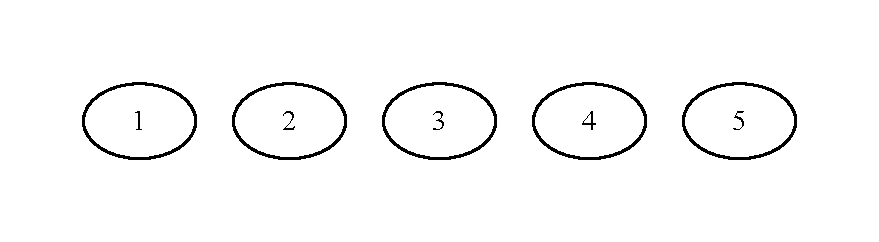
\includegraphics[width=0.6\textwidth]{images/randomgraph-01.pdf}
\caption{RandomGraph, stap 1}
\label{fig:randomgraph-01}
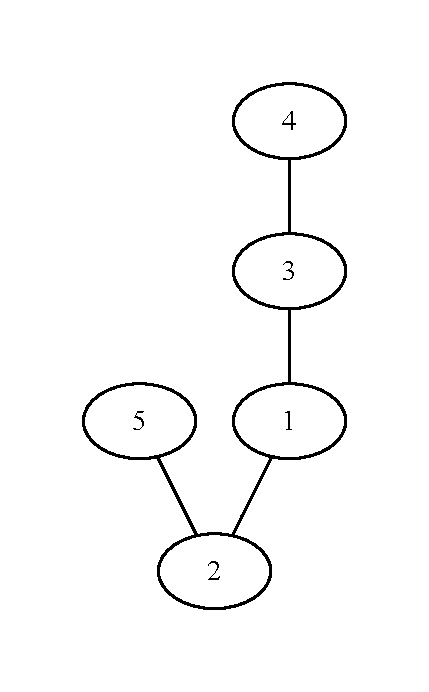
\includegraphics[width=0.3\textwidth]{images/randomgraph-02.pdf}
\caption{RandomGraph, stap 2}
\label{fig:randomgraph-02}
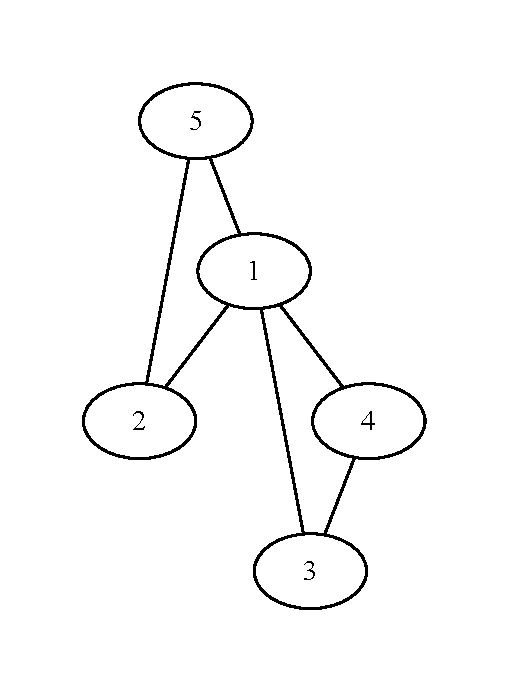
\includegraphics[width=0.3\textwidth]{images/randomgraph-03.pdf}
\caption{RandomGraph, stap 3}
\label{fig:randomgraph-03}
\end{center}
\end{figure}

\section{Het na\"ieve algoritme}

\subsection{Lazy genereren van embeddingen}
Ons na\"ieve algoritme overloopt alle embeddingen. Het is echter belangrijk dat
we de embeddingen op een \emph{lazy} manier genereren. Indien we de permutaties
\emph{strict} zouden genereren, zouden we een algoritme krijgen dat (weliswaar
met branching) het volgende idee implementeerd:

\lstset{language=Python}
\begin{lstlisting}
genus = +Infinity
for e in getEmbeddings(graph):
    eGenus = getGenus(e)
    if eGenus < genus:
        genus = eGenus
\end{lstlisting}

Hierbij is het probleem dat we pas informatie over het genus krijgen op het
moment dat e gegenereerd is. Als we hierop bounding criteria willen toepassen,
zouden we enkel de bladeren in onze zoekboom kunnen schrappen. Omdat we meer
willen schrappen, zoeken we dus naar een beter algoritme, waarin we vroeger
informatie over het genus verkrijgen.
\newline

\subsection{findGenus en findFaces}
Het genus van een graaf en een embedding $i$ wordt gegeven door
$v + f_i - e = 2 - 2g_i$. We weten $v$ en $e$ vast liggen, en enkel $f$ vari\"eert
als voor een graaf de embeddingen aflopen. Het zoeken van $min(g)$ komt dus
neer op het zoeken van $max(f)$, want
\begin{equation*}
min(g) = 1 - \frac{v + max(f) - e}{2}
\end{equation*}

\subsection{Algoritme: Het zoeken van het maximaal aantal vlakken}
Eerst zetten we de graaf die we krijgen als input om in een gerichte graaf. We
beginnen met een willekeurige (gerichte) boog $e_1$ die nog niet in een pad
ligt.  Stel dat op het einde van deze boog de top $v$ ligt. We nemen nu de
verzameling kandidaat bogen $E_v$ die op $e_i$ kunnen volgen. Deze stap is niet
triviaal en wordt verder beschreven in \ref{kandidaatbogen}. Nu moeten we branchen
voor elk element van $E_v$. We voegen de gekozen boog $e_{i+1}$ toe aan ons pad.
Indien deze boog dezelfde boog is als de eerste boog in ons pad, $e_1$, Hebben
we van ons pad een cykel gemaakt. Op dat moment kijken we of er nog bogen zijn
die niet in een pad liggen. Als dit het geval is, beginnen we een nieuw pad met
een willeukerige boog. Anders hebben we een volledige embedding gevonden, en
bevinden we ons in een blad van de zoekboom.
\newline

\subsection{Het nemen van kadidaatbogen volgend op een boog}
\label{kandidaatbogen}
Onze embedding defini\"eert voor elke top een bepaalde volgorde van de bogen in
deze top. We slaan deze volgordes op in de klasse \verb#CycleNode#. Initieel kan
elke boog volgen op elke andere boog. We stellen dit voor als $n$ deelvolgordes
\begin{equation*}
(e_1) (e_2) (e_3) \dots (e_n)
\end{equation*}
voor een top met $n$ bogen. Stel dat we op een bepaald moment in ons algoritme
in de top toekomen via $e_i$ en weggaan via $e_j$. Vanaf dit moment moeten we
hiermee rekening houden, mochten we nog eens in de top komen. We slaan dit op
als
\begin{equation*}
(e_1) (e_2) (e_3) \dots (e_i e_j) \dots (e_n)
\end{equation*}
Hoe vinden we nu de kandidaatbogen? Stel dat we uit $e_i$ komen. We hebben in
onze top de volgende volgordes opgeslaan:
\begin{equation*}
(e_{a1} e_{a2} \dots e_{ax}) (e_{b1} e_{b2} \dots e_{by}) \dots (e_{c1} e_{c2} \dots e_{cz})
\end{equation*}
We weten dat er nog geen boog volgt op $e_i$, dus zal $e_i$ het laatste element
zijn in een deelvolgorde.
\newline

We kunnen bijvoorbeeld niet $e_{a2}$ als volgende boog kiezen, omdat we al
gedefini\"eerd hebben dat deze op $e_{a1}$ volgt. Stel dat $e_i = e_{ax}$,
dan kunnen we niet als volgende boog $e_{a1}$ kiezen, want op dat moment zouden
we de deelvolgorde \emph{sluiten}. Dit mag niet, want, zoals in de opgave
beschreven wordt, moeten we uiteindelijk een volgorde als $(e_1 e_2 \dots e_n)$
uitkomen, zodat als we de volgorde doorlopen, elke $e$ tegenkomen.
\newline

Meer algemeen zijn de deelkandidaten die kunnen volgen op $e_i$ alle $e_j$ die
voldoen aan twee voorwaarden:
\begin{itemize}
\item $e_j$ is het eerste element van een deelvolgorde
$(e_j e_{j+1} ... e_{j+n})$.
\item $e_j$ zit niet in dezelfde deelvolgorde als $e_i$.
\end{itemize}

Een uitzondering bestaat wanneer we slechts \'e\'en deelvolgorde 
$(e_1 e_2 \dots e_i)$ ($e_i$ is dan het laatste element, aangezien het als
enige $e$ nog geen opvolger heeft) meer hebben. Dit geval is echter triviaal,
dan is de enige kandidaat $e_1$.

\section{Bounding Criteria}

\subsection{Een ondergrens voor het maximaal aantal vlakken}
\label{ondergrens-maximaal-aantal-vlakken}
We kunnen bounden als we een ondergrens $m$ hebben voor het maximaal aantal
vlakken $F$. We zoeken immers $F$. Stel dat we in het algoritme zitten en we
hebben momenteel $f$ vlakken. We hebben eerder al een embedding gevonden met
$m$ vlakken. Stel dat we weten dat we $x$ vlakken kunnen maken met de bogen die
we op dat moment nog niet gebruikt hebben. Dat betekent dat we kunnen stoppen
met ons algoritme zodra
\begin{equation*}
f + x \leq m
\end{equation*}
want we weten dat
\begin{equation*}
m \leq F
\end{equation*}
en dus
\begin{equation*}
f + x \leq F
\end{equation*}
Dit laatste impliceert dat we toch geen embedding met meer vlakken zullen vinden
in de huidige branch van de zoekruimte, en dus kunnen we maar beter stoppen.
\newline

Het is nu de vraag hoe we $x$ kiezen. Om ons algoritme performant te maken,
willen we veel bounden, en dus willen we dat $f + x < m$ zoveel mogelijk
voorkomt. We willen $x$ dus zo klein mogelijk, maar natuurlijk nog altijd
correct, omdat we niet te vroeg willen bounden. We willen natuurlijk ook niet
te veel tijd besteden aan $x$ te berekenen, omdat zo het voordeel dat we krijgen
door bounding weer zal wegvallen.

\subsection{Pariteit van het aantal vlakken}
Als we de formule
\begin{equation*}
g = 1 - \frac{v + f - e}{2}
\end{equation*}
bekijken, en we weten dat $g$ altijd een geheel getal is, kunnen we hieruit
afleiden dat $v + f - e$ altijd even is. Dit betekend dat, aangezien $v$ en $e$
vastliggen voor de graaf, $f$ dezelfde pariteit zal behouden. Met andere
woorden, vinden we een embedding $E_1$ met $f_1$ vlakken, en een embedding $E_2$
met $f_2$ vlakken, dan weten we dat ofwel $f_1$ en $f_2$ beide even zijn, ofwel
beide oneven.

Als we ons boundingcriteria uit \ref{ondergrens-maximaal-aantal-vlakken}
bekijken,
\begin{equation*}
f + x \leq m
\end{equation*}
kunnen we dit nog verbeteren. Stel immers dat er een embedding kan gevonden met
aantal vlakken $f_1$ zodat $f_1 > m$. Aangezien $m$ ook een aantal vlakken
gevonden in een embedding voorstelt, zal wegens het feit dat $f_i$ en $m$
dezelfde pariteit bezitten ook gelden dat $f_1 > m + 1$. We kunnen dus nog iets
sneller bounden, namelijk zodra
\begin{equation*}
f + x \leq m + 1
\end{equation*}

\subsection{Een eerste poging}
\label{een-eerste-poging}
We weten dat we om een vlak te maken tenminste 3 bogen nodig hebben. We
houden dus het aantal bogen dat we nog niet gebruikt hebben bij in $l$. We vinden
dan dat
\begin{equation*}
x = \lfloor \frac{max(2, c) + l}{3} \rfloor
\end{equation*}
met $c$ het aantal bogen in de huidige cykel. We tellen $max(2, c)$ op bij $l$
omdat we zo $x$ preciezer maken. Als we al meer dan 2 bogen in de huidige
cykel hebben, kunnen we met 1 boog uit $l$ een extra cykel maken. Anders
hebben we er $3 - c$ nodig. Dit zit op deze manier ook in onze berekening.

\subsection{Girth van een graaf}
In \ref{een-eerste-poging} gingen we ervan uit dat we tenminste 3 bogen nodig
hebben om een vlak te maken. Dit is natuurlijk altijd waar, maar stel dat we
een graaf hebben als in Figuur \ref{fig:cube}. Als we deze graaf bekijken, zien
we dat we tenminste 4 bogen nodig hebben om een vlak te maken. Aan de hand van
deze informatie kunnen we een betere $x$ opstellen voor deze graaf.
\begin{equation*}
x = \lfloor \frac{max(3, c) + l}{4} \rfloor
\end{equation*}
We vragen ons natuurlijk af hoe we dit algemeen kunnen toepassen. Het
\emph{girth} van een graaf is de lengte van kleinste cykel. Dit is precies wat
we nodig hebben! We kunnen dus voor elke graaf schrijven:
\begin{equation*}
x = \lfloor \frac{max(girth - 1, c) + l}{girth} \rfloor
\end{equation*}
Hoe moeten we het \emph{girth} van een graaf nu berekenen? We kiezen voor een
eenvoudige manier. We starten vanuit elke top van de graaf een
\emph{breadth-first search} en houden de diepte bij. Op het moment dat we een
top terechtkomen waar we al geweest zijn, hebben we de kleinste cykel van de
graaf gevonden waar de wortel van de BFS in ligt. Door een BFS te starten vanuit
elke top, kunnen we de kleinste cykel van de gehele graaf bepalen.  Dit
algoritme is ge\"implementeerd in de klasse \verb#FindGirth#.
\newline

In het slechtste geval moet de BFS voor elke top de gehele graaf doorzoeken. De
tijdscomplexiteit voor dit algoritme wordt dus naar boven begrensd door $O(ve)$
met $v$ het aantal vertices, en $e$ het aantal (ongerichte) bogen.

\begin{figure}
\begin{center}
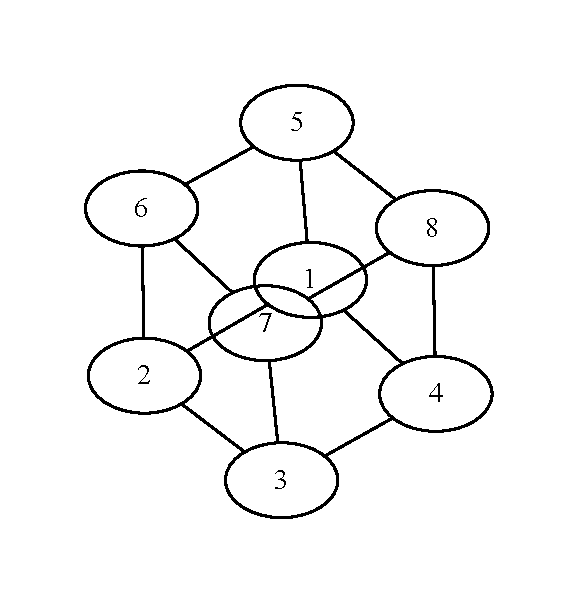
\includegraphics[width=0.4\textwidth]{images/cube.pdf}
\caption{Een graaf met \emph{girth} 4}
\label{fig:cube}
\end{center}
\end{figure}


\section{Heuristieken}

\subsection{Een smalle stam voor de zoekboom}
We willen een zoekboom die een smalle stam heeft en een brede kruin (zoals in
Figuur \ref{fig:good-tree}), in plaats van een zoekboom met een brede stam en
een smalle kruin (zoals in Figuur \ref{fig:bad-tree}). Met andere woorden, we
willen dat ons algoritme in het begin zo weinig mogelijk moet branchen, en
naarmate we dieper in de zoekboom afdalen, mag het meer branchen.
\newline

Het voordeel hiervan is dat wanneer we delen van de zoekboom mogen uitschakelen,
meestal grotere delen kunnen uitschakelen.
\newline

\begin{figure}
\begin{center}
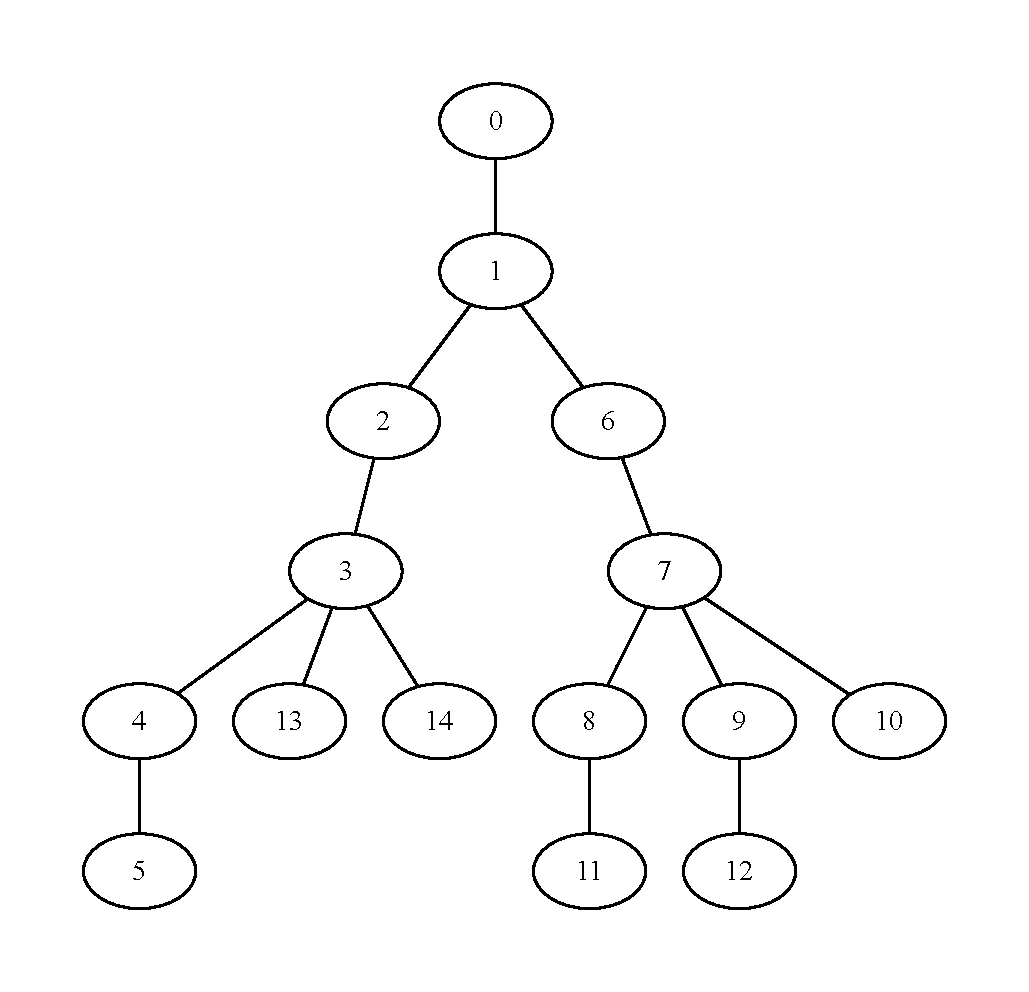
\includegraphics[width=0.6\textwidth]{images/good-tree.pdf}
\caption{Een boom met een smalle stam en een brede kruin}
\label{fig:good-tree}
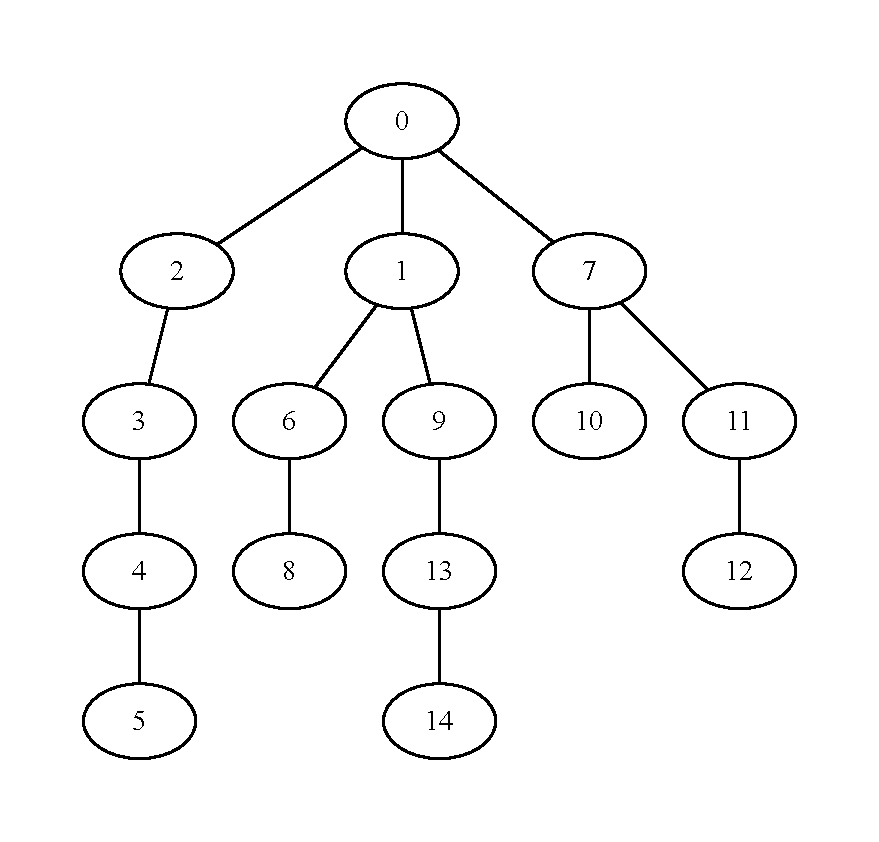
\includegraphics[width=0.6\textwidth]{images/bad-tree.pdf}
\caption{Een boom met een brede stam en een smalle kruin}
\label{fig:bad-tree}
\end{center}
\end{figure}

De vraag is natuurlijk hoe we onze zoekboom een zodanige vorm kunnen geven. Dit
is echter vrij eenvoudig. We weten dat ons algoritme zal branchen als we in een
top staan, en er zijn meerdere kandidaatbogen. Het aantal branches wordt
natuurlijk bepaald door het aantal kandidaatbogen. Het aantal kandidaatbogen is
dan weer grotendeels afhankelijk van het aantal bogen in die top.
\newline

We willen dus dat ons algoritme eerst de toppen bezoekt met veel bogen, en
vervolgens de toppen met minder bogen. Dit implementeren we door de toppen van
de graaf te sorteren op het aantal bogen.
\newline

Dit versneld ons algoritme voor bepaalde grafen. Het zal uiteraard niets
uitmaken bij zeer regelmatige grafen zoals de complete grafen, aangezien er daar
in elke top ongeveer evenveel bogen zijn. Maar aangezien het sorteren relatief
snel kan gebeuren, is het toch de moeite waard om deze heuristiek te gebruiken.
\newline

Voor willeukeurig gevormde grafen scheelt het immers wel.

\end{document}
